\chapter{Appendices}
In the following pages a subset of all the code, plots and data generated in this project is presented. As hundreds of plots have been created it was an impossible task to get them all included in the appendices. If some specific code or plot or data is missing, it can all be found at \githuburl{}. The sessions subfolder contains most of what could be interesting to look at.
\vspace{\stretch{1}}
\pagebreak

\section{Splitting dataset} % (fold)
\label{app:source-splitting-data}
\githublisting{../}{src/create_test_and_training_data_set.py}
% section  (end)

\clearpage

\section{Calculating common statistics - Code}\label{app:source-common-statistics}
\lstinputlisting[caption=\githuburl{sessions/9-data-exploration/src/calculate_summary_statistics.py}]{../sessions/9-data-exploration/src/calculate_summary_statistics.py}

\vspace{\stretch{1}}

\pagebreak

\section{Calculating common statistics - Result}\label{app:result-common-statistics}
{\small\sffamily
\begin{python}
    import scripts.commonstats_table as c; c.render('../sessions/9-data-exploration/src/summary_statistics.json')
\end{python}
}

\clearpage

\section{Calculate unique values of features - Code} % (fold)
\label{app:source-unique-values}
\lstinputlisting[caption=\githuburl{sessions/9-data-exploration/src/calculate_unique_values.py}]{../sessions/9-data-exploration/src/calculate_unique_values.py}
\lstinputlisting[caption=\githuburl{sessions/9-data-exploration/src/calculate_unique_values_pr_trial.py}]{../sessions/9-data-exploration/src/calculate_unique_values_pr_trial.py}
\lstinputlisting[caption=\githuburl{sessions/9-data-exploration/src/unique_values_combined.py}]{../sessions/9-data-exploration/src/unique_values_combined.py}
% section Calculate unique values of features (end)

\clearpage

\section{Calculate unique values of features - Result} % (fold)
\label{app:result-unique-values}
{\small\sffamily
\begin{python}
    import scripts.uniquevalues_table as c; c.render()
\end{python}
}
% section Calculate unique values of features - Result (end)

\clearpage

\section{Creating boxplots - Code} % (fold)
\label{app:source-boxplots}
\githublisting{../}{sessions/11-boxplots-scatterplots/scripts/create_boxplots.py}
% section Creating boxplots - Code (end)

\clearpage

\section{Creating boxplots - Result} % (fold)
\label{app:result-boxplots}
All boxplots can be found at \githuburl{sessions/11-boxplots-scatterplots/plots/boxplots}
% section Creating boxplots - Result (end)

\clearpage

\section{Creating layered feature plots - Code} % (fold)
\label{app:source-layered-feature-plots}
\githublisting{../}{sessions/22-create-transparent-feature-plots/scripts/create_plots_random_trials.py}
\githublisting{../}{sessions/22-create-transparent-feature-plots/scripts/create_naive_plots.py}
% section Creating layered featuer plots - Code (end)

\clearpage

\section{Creating layered feature plots - Result} % (fold)
\label{app:result-layered-feature-plots}
\begin{figure}[hb]
    \centering
    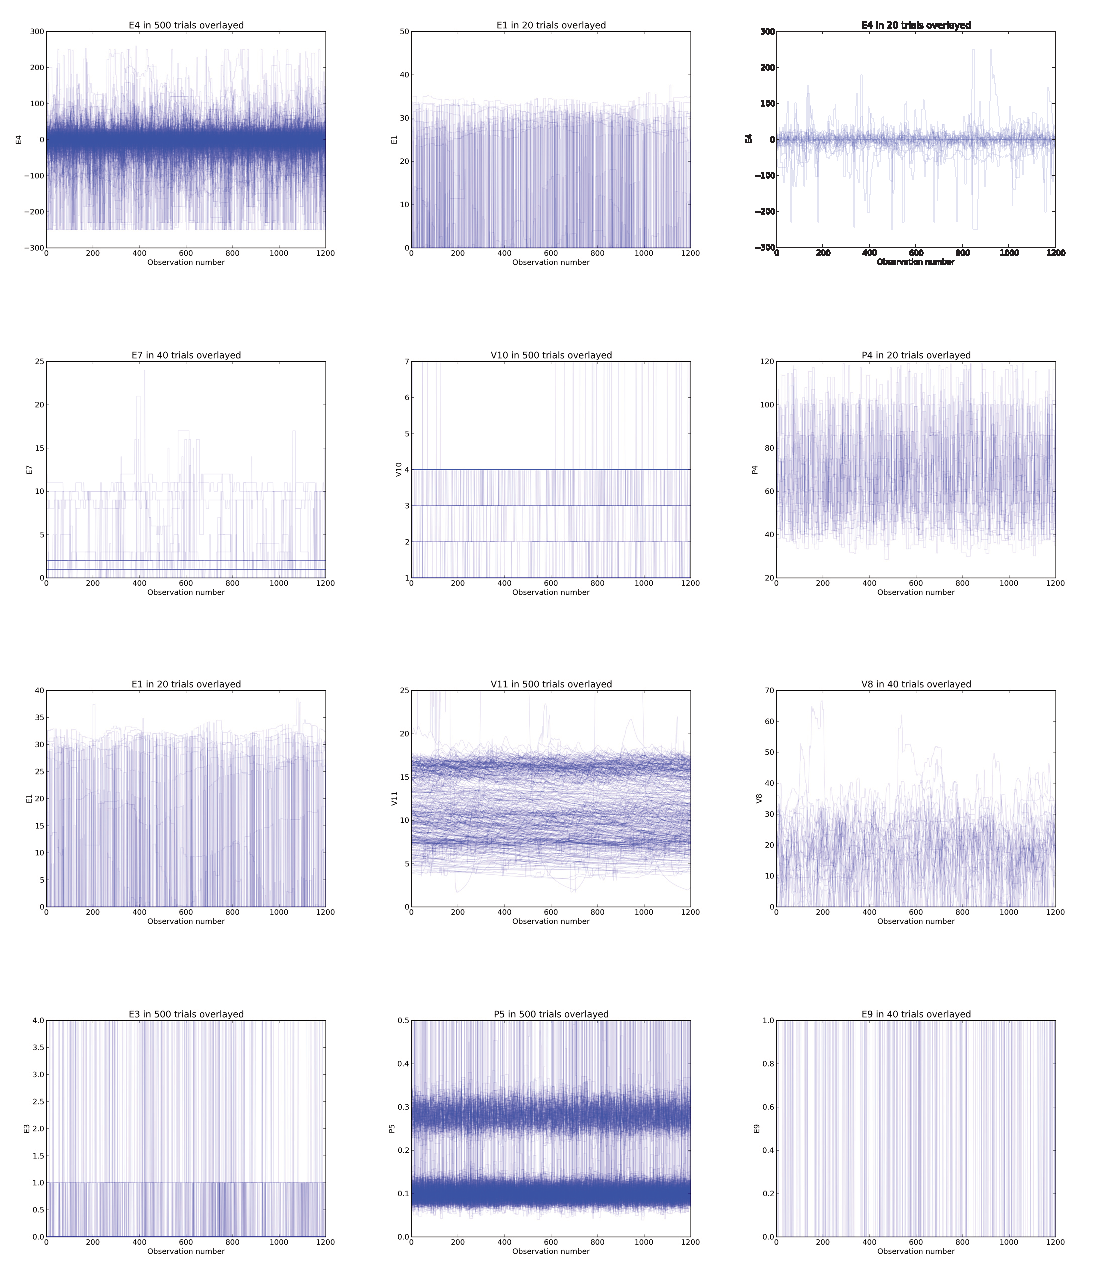
\includegraphics[width=.9\textwidth]{media/layered-plots-sheet.pdf}
    \caption{}
\end{figure}
% section Creating layered feature plots - Result (end)

\clearpage

\section{Scatterplots - Code} % (fold)
\label{app:source-scatterplots}
\githublisting{../}{sessions/24-writing-helper-scripts/scripts/rewrite-scatterplot-script.py}
% section source-scatterplots (end)

\clearpage

\section{Scatterplots - Result} % (fold)
\label{app:result-scatterplots}
\begin{figure}[hb]
    \centering
    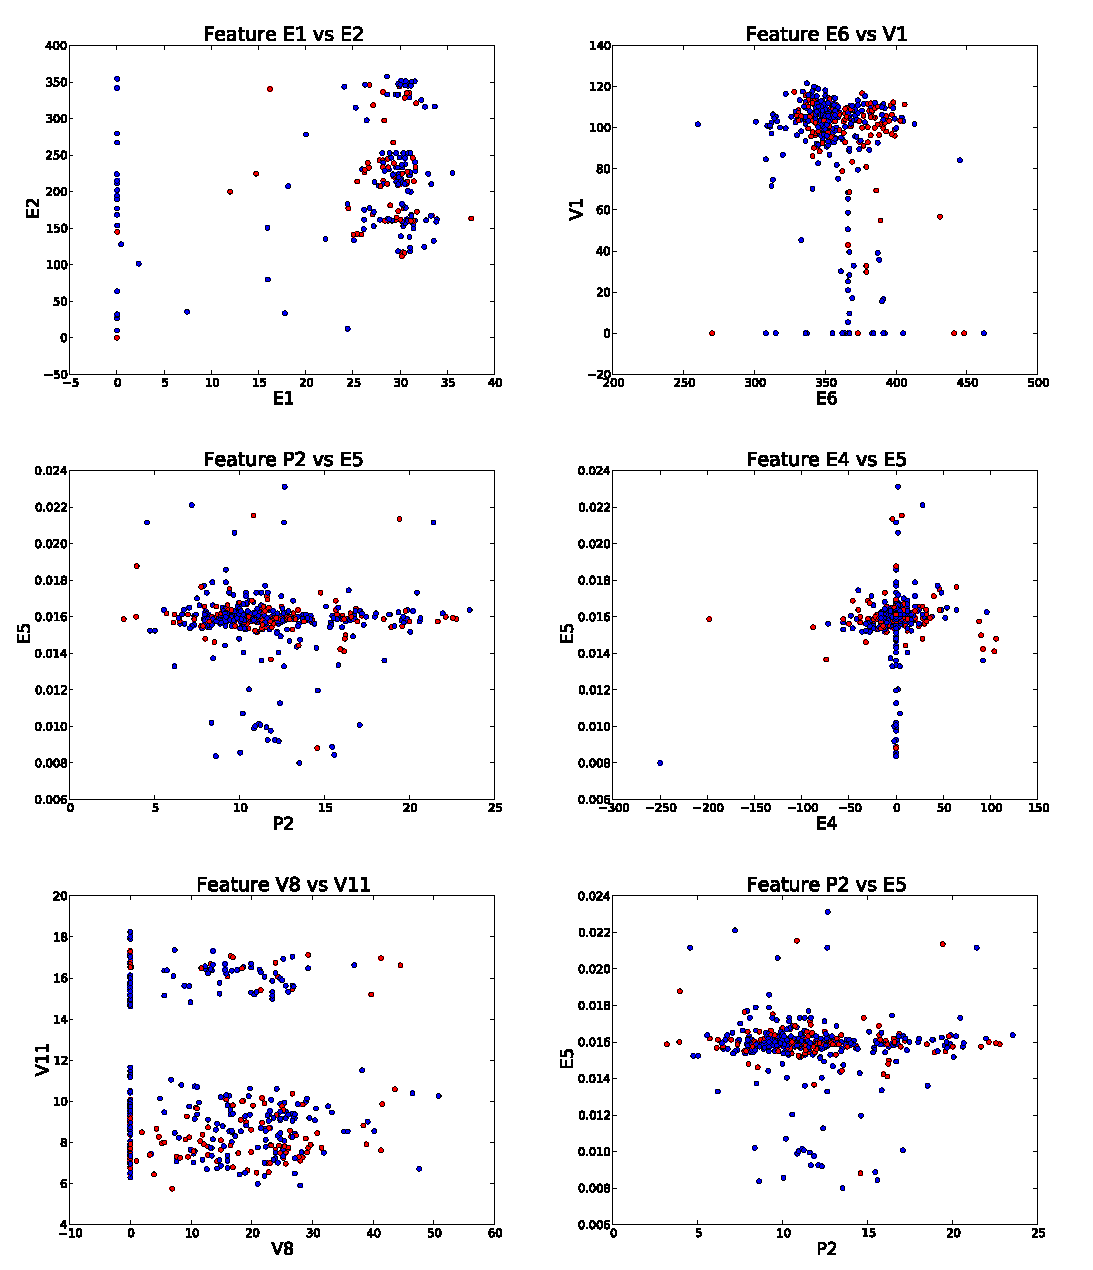
\includegraphics[width=.9\textwidth]{media/scatterplots-sheet.pdf}
    \caption{}
\end{figure}
% section  (end)

\clearpage

\section{Recreating the winning approach - Code} % (fold)
\label{app:source-recreate-winner}
\githublisting{../}{sessions/17-recreating-winning-entry/scripts/inferences_features_cv_2.py}

\section{Helper functions for logistic regression - Code} % (fold)
\label{app:helper-logistic}
\githublisting{../}{src/logistic.py}
% section Recreating the winning approach - Code (end)

\clearpage

\section{Forward selection - Code} % (fold)
\label{app:source-forward-selection}
\githublisting{../}{sessions/18-forward-selection/scripts/forward_selection.py}
% section  (end)

\clearpage

\section{Forward selection - Results} % (fold)
\label{app:result-forward-selection}
{\small\sffamily\centering
\begin{minipage}[t]{40mm}
\vspace{0pt}
\begin{tabularx}{40mm}{ l R }
Feature added & AUC \\\hline
V11 & 0.6978 \\
E9 & 0.8089 \\
sdE1 & 0.8333 \\
mE6 & 0.8500 \\
sdE4 & 0.8539 \\
mV3 & 0.8566 \\
sdV8 & 0.8597 \\
E8 & 0.8612 \\
mE10 & 0.8623 \\
mP5 & 0.8635 \\
sdP5 & 0.8687 \\
mP7 & 0.8705 \\
mV11 & 0.8717 \\
V10 & 0.8727 \\
sdV1 & 0.8737 \\
mE4 & 0.8744 \\
sdP2 & 0.8759 \\
sdE6 & 0.8766 \\
sdP7 & 0.8771 \\
sdP1 & 0.8778 \\
sdE2 & 0.8781 \\
mV2 & 0.8785 \\
mE8 & 0.8790 \\
sdV10 & 0.8793 \\
{\itshape continues ...} & 
\end{tabularx}
\end{minipage}
\hspace{35mm}
\begin{minipage}[t]{40mm}
\vspace{0pt}
\begin{tabularx}{40mm}{ l R }
Feature added & AUC \\\hline
{\itshape ... continued} \\
sdV3 & 0.8799 \\
sdE9 & 0.8802 \\
sdE8 & 0.8811 \\
mE7 & 0.8818 \\
mE9 & 0.8822 \\
mV4 & 0.8827 \\
mV5 & 0.8832 \\
mE1 & 0.8833 \\
E6 & 0.8835 \\
V4 & 0.8839 \\
V2 & 0.8839 \\
E10 & 0.8840 \\
V5 & 0.8841 \\
sdE3 & 0.8843 \\
sdE11 & 0.8843 \\
P4 & 0.8844 \\
mE11 & 0.8846 \\
sdP4 & 0.8848 \\
sdV2 & 0.8848 \\
sdV4 & 0.8849 \\
mV8 & 0.8851 \\
mV6 & 0.8855 \\
mP1 & 0.8857 \\
sdE5 & 0.8858 \\
\end{tabularx}
\end{minipage}
}
% section  (end)

\clearpage

\section{Neural Network - Code} % (fold)
\label{app:source-neural-network}
\githublisting{../}{sessions/25-neural-network/scripts/inference-features.py}
% section section name (end)


\clearpage

\section{Create extended dataset function - Code} % (fold)
\label{sec:Create extended dataset function - Code}
\lstinputlisting[caption={Function to create extended dataset. Part of the file \githuburl{src/utils2.py}}]{media/create_extended_dataset.py}
% section Create extended dataset function - Code (end)

\clearpage

\section{Original timeschedule} % (fold)
\label{app:timeschedule}
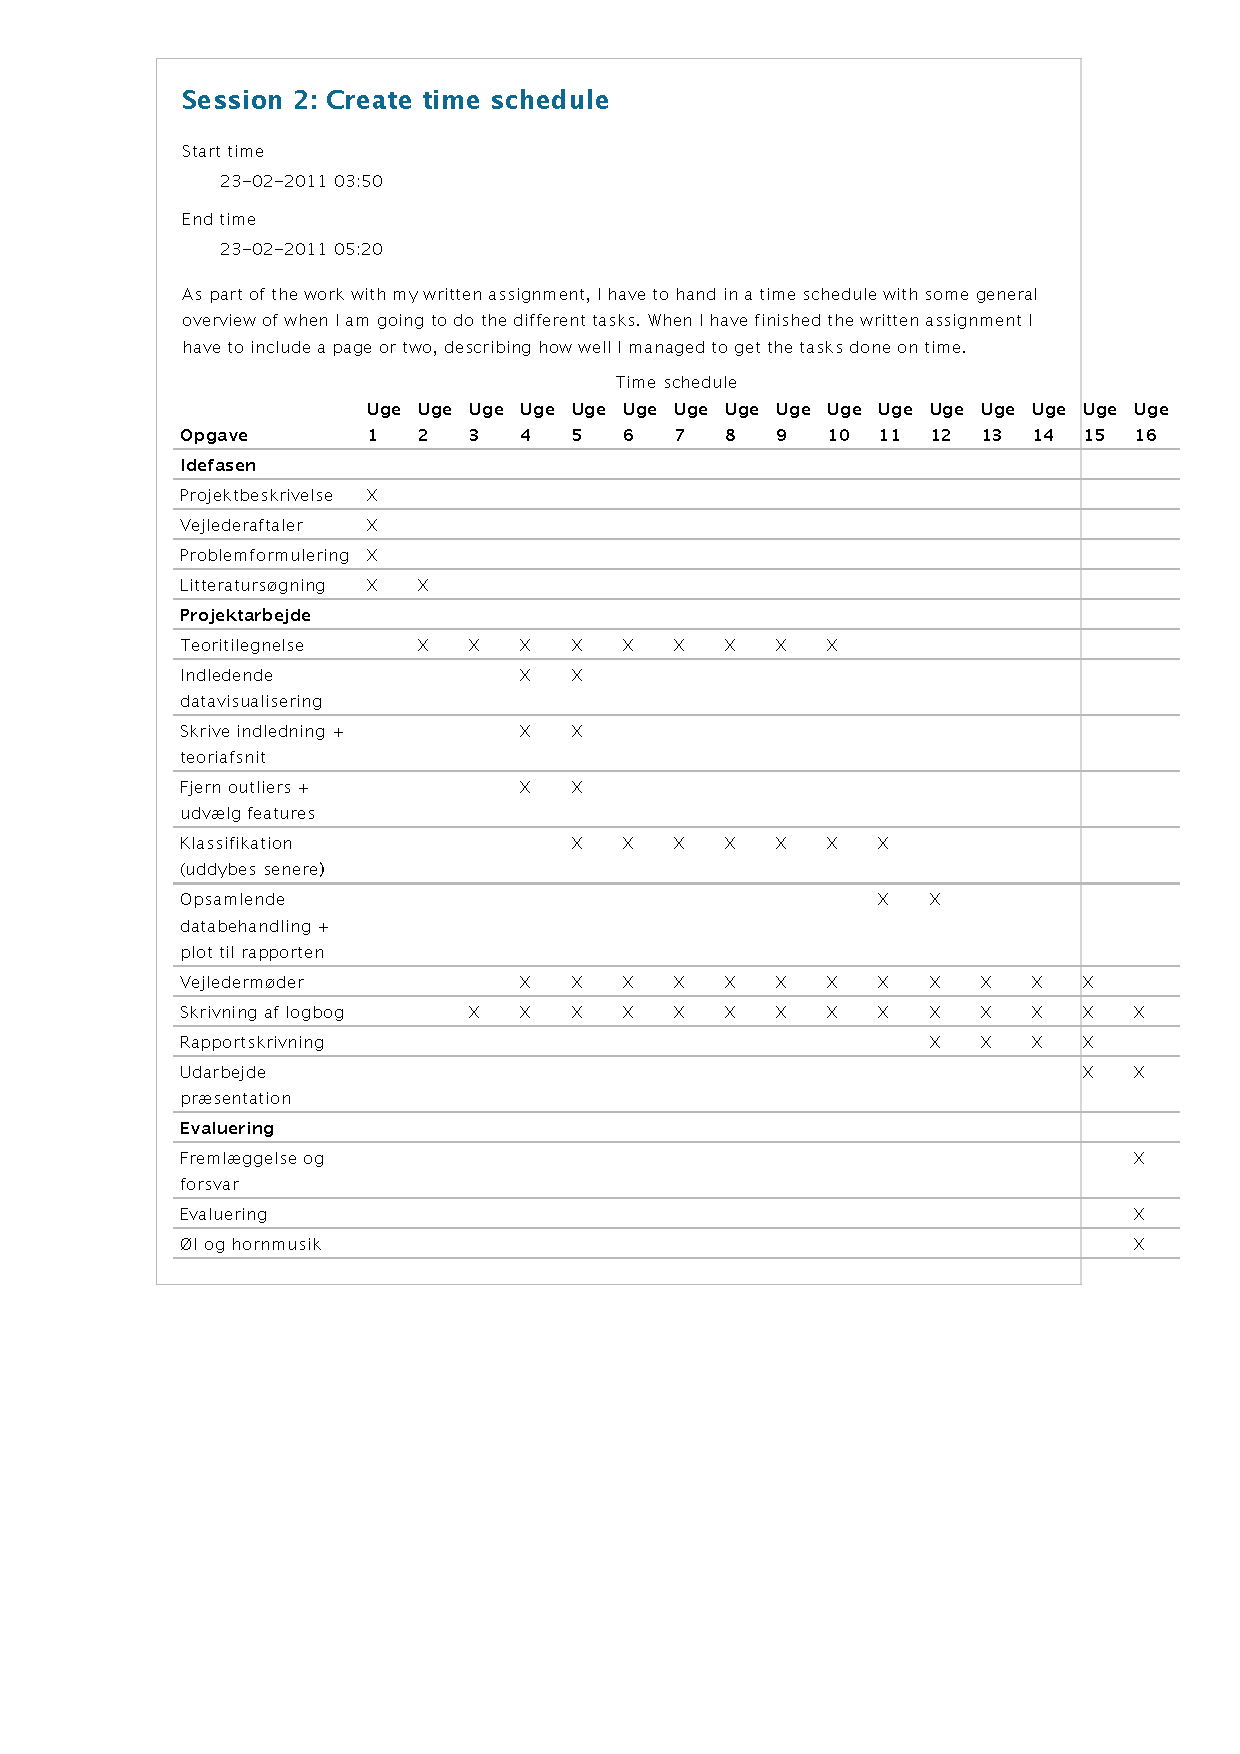
\includegraphics[width=120mm]{media/timeschedule.pdf}
% section Original timeschedule (end)
